\subsection{Analisi preliminare, verifica delle leggi di Fresnel}\label{subsec:analisi-dati}
  In questo modo, abbiamo ottenuto le misure di intensità riflessa $I_\pi$ e $I_\sigma$ [fig ??]. Per ottenere i
  coefficienti di Fresnel, abbiamo normalizzato i dati ottenuti tenendo conto che:
  there is no difference between Rp and Rs at normal incidence
  at glancing angle in the less-dense medium the reflection coefficients are ±1,
  Come descritto in [Lipson]
  Da queste misure abbiamo ricavato anche l’angolo di Brewster, osservando per quale valore di $\theta_i$
  l’intensità $I_\pi$ si annulla.
  %TODO

  \begin{figure}[h]
    \centering
    \caption{Sburino}
    \begin{subfigure}{.4\textwidth}
      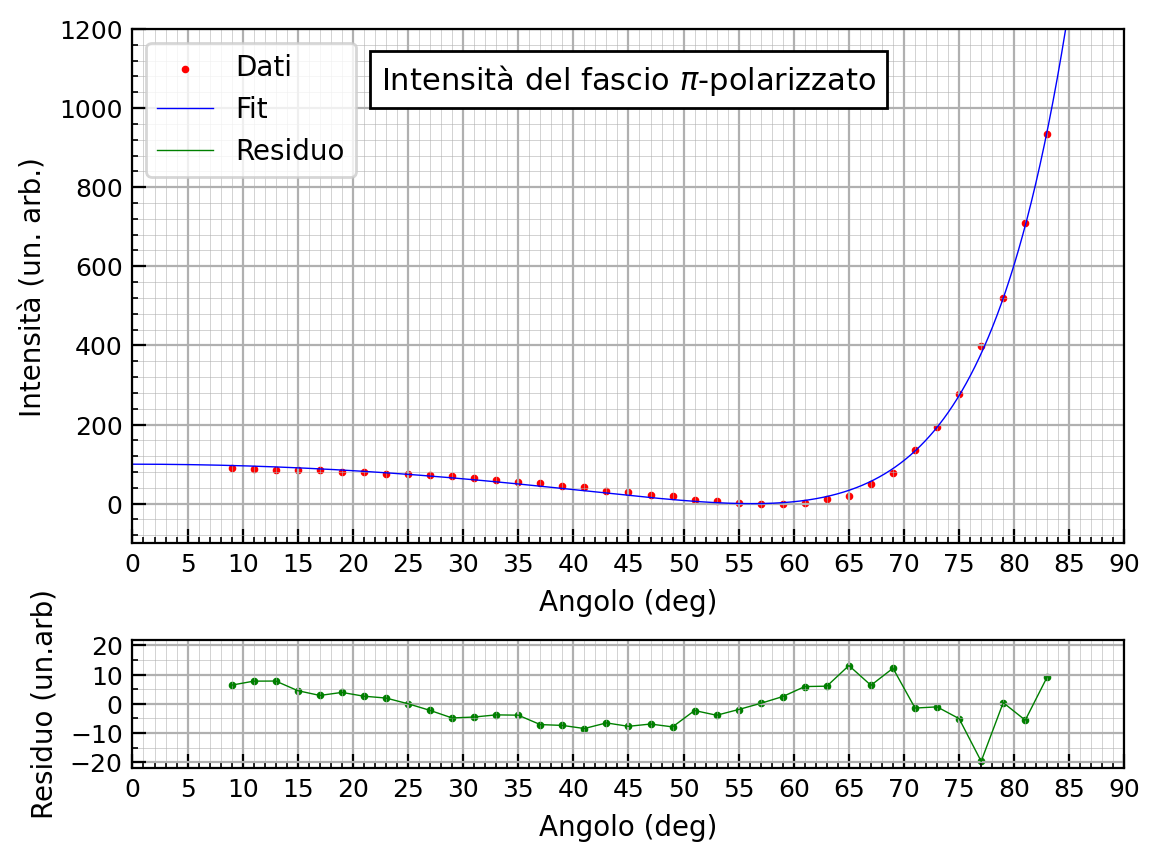
\includegraphics[width=7cm]{./graphs/raw-pi.png}
      \caption{
        \emph{
          sbüro
        }
      }
      \label{fig:raw-pi}
    \end{subfigure}%
    \hspace{20mm}
    \begin{subfigure}{.4\textwidth}
      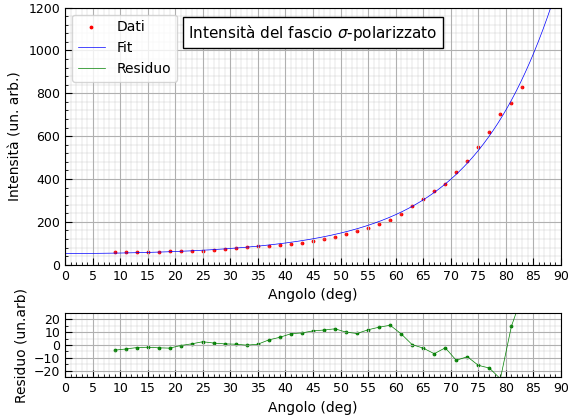
\includegraphics[width=7cm]{./graphs/raw-sigma.png}
      \caption{
        \emph{
          sbruña
        }
      }
      \label{fig:raw-sigma}
    \end{subfigure}
  \end{figure}
\subsection{Misura dell'angolo di Brewster}\label{subsec:angolo-di-brewster}
  \blindtext[2]
  % TODO
\endinput



